\documentclass[a4paper, 14pt]{extarticle}

% Поля
%--------------------------------------
\usepackage{geometry}
\geometry{a4paper,tmargin=2cm,bmargin=2cm,lmargin=3cm,rmargin=1cm}
%--------------------------------------

\usepackage{float}
%Russian-specific packages
%--------------------------------------
\usepackage[T2A]{fontenc}
\usepackage[utf8]{inputenc} 
\usepackage[english, main=russian]{babel}
%--------------------------------------

\usepackage{textcomp}
\usepackage{xcolor}

% Красная строка
%--------------------------------------
\usepackage{indentfirst}               
%--------------------------------------
%Листинги
%--------------------------------------
\usepackage{listings}
\lstset{
  basicstyle=\ttfamily\footnotesize,
  breakatwhitespace=false,
  breaklines=true,
  captionpos=t,
  inputencoding=utf8,
  extendedchars=true,
  literate={а}{а}1{б}{б}1{в}{в}1{г}{г}1{д}{д}1{е}{е}1{ё}{ё}1{ж}{ж}1{з}{з}1{и}{и}1{й}{й}1{к}{к}1{л}{л}1{м}{м}1{н}{н}1{о}{о}1{п}{п}1{р}{р}1{с}{с}1{т}{т}1{у}{у}1{ф}{ф}1{х}{х}1{ц}{ц}1{ч}{ч}1{ш}{ш}1{щ}{щ}1{ъ}{ъ}1{ы}{ы}1{ь}{ь}1{э}{э}1{ю}{ю}1{я}{я}1,
  frame=single,
  keepspaces=true,
  keywordstyle=\bf,
  numbers=none,
  xleftmargin=25pt,
  xrightmargin=25pt,
  showspaces=false,
  showstringspaces=false,
  showtabs=false,
  stepnumber=1,
  tabsize=2,
  title=\lstname
}
%--------------------------------------
\usepackage[most]{tcolorbox}
\tcbuselibrary{listings,breakable}
\newtcblisting{breakablelisting}{
  listing only,
  breakable,
  enhanced,
  frame hidden,
  colback=white,
  left=8pt,
  overlay={\draw[line width=0.4pt] (frame.north west) -- (frame.south west);
          \draw[line width=0.4pt] ([xshift=3pt]frame.north west) -- ([xshift=3pt]frame.south west);},
  listing options={
    frame=none,
    numbers=none,
    mathescape=false,
    texcl=false,
    inputencoding=utf8,
    extendedchars=true,
    literate={а}{а}1{б}{б}1{в}{в}1{г}{г}1{д}{д}1{е}{е}1{ё}{ё}1{ж}{ж}1{з}{з}1{и}{и}1{й}{й}1{к}{к}1{л}{л}1{м}{м}1{н}{н}1{о}{о}1{п}{п}1{р}{р}1{с}{с}1{т}{т}1{у}{у}1{ф}{ф}1{х}{х}1{ц}{ц}1{ч}{ч}1{ш}{ш}1{щ}{щ}1{ъ}{ъ}1{ы}{ы}1{ь}{ь}1{э}{э}1{ю}{ю}1{я}{я}1,
    literate={\$}{{\$}}1
  }
}


%Graphics
%--------------------------------------
\usepackage{graphicx}
\usepackage{wrapfig}
%--------------------------------------
\graphicspath{{./lab5/}{./}}
% Полуторный интервал
%--------------------------------------
\linespread{1.3}                    
%--------------------------------------

%Выравнивание и переносы
%--------------------------------------
% Избавляемся от переполнений
\sloppy
% Запрещаем разрыв страницы после первой строки абзаца
\clubpenalty=10000
% Запрещаем разрыв страницы после последней строки абзаца
\widowpenalty=10000
%--------------------------------------

%Списки
\usepackage{enumitem}

%Подписи
\usepackage{caption} 

%Гиперссылки
\usepackage{hyperref}

\hypersetup {
	unicode=true
}

%Рисунки
%--------------------------------------
\DeclareCaptionLabelSeparator*{emdash}{~--- }
\captionsetup[figure]{labelsep=emdash,font=onehalfspacing,position=bottom}
%--------------------------------------

\usepackage{tempora}

%--------------------------------------

%%% Математические пакеты %%%
%--------------------------------------
\usepackage{amsthm,amsfonts,amsmath,amssymb,amscd}  % Математические дополнения от AMS
\usepackage{mathtools}                              % Добавляет окружение multlined
\usepackage[perpage]{footmisc}
%--------------------------------------

%--------------------------------------
%			НАЧАЛО ДОКУМЕНТА
%--------------------------------------

\begin{document}

%--------------------------------------
%			ТИТУЛЬНЫЙ ЛИСТ
%--------------------------------------
\begin{titlepage}
\thispagestyle{empty}
\newpage


%Шапка титульного листа
%--------------------------------------
\vspace*{-60pt}
\hspace{-65pt}
\begin{minipage}{0.3\textwidth}
\hspace*{-20pt}\centering
\includegraphics[width=\textwidth]{emblem}
\end{minipage}
\begin{minipage}{0.67\textwidth}\small \textbf{
\vspace*{-0.7ex}
\hspace*{-6pt}\centerline{Министерство науки и высшего образования Российской Федерации}
\vspace*{-0.7ex}
\centerline{Федеральное государственное автономное образовательное учреждение }
\vspace*{-0.7ex}
\centerline{высшего образования}
\vspace*{-0.7ex}
\centerline{<<Московский государственный технический университет}
\vspace*{-0.7ex}
\centerline{имени Н.Э. Баумана}
\vspace*{-0.7ex}
\centerline{(национальный исследовательский университет)>>}
\vspace*{-0.7ex}
\centerline{(МГТУ им. Н.Э. Баумана)}}
\end{minipage}
%--------------------------------------

%Полосы
%--------------------------------------
\vspace{-25pt}
\hspace{-35pt}\rule{\textwidth}{2.3pt}

\vspace*{-20.3pt}
\hspace{-35pt}\rule{\textwidth}{0.4pt}
%--------------------------------------

\vspace{1.5ex}
\hspace{-35pt} \noindent \small ФАКУЛЬТЕТ\hspace{80pt} <<Информатика и системы управления>>

\vspace*{-16pt}
\hspace{47pt}\rule{0.83\textwidth}{0.4pt}

\vspace{0.5ex}
\hspace{-35pt} \noindent \small КАФЕДРА\hspace{50pt} <<Теоретическая информатика и компьютерные технологии>>

\vspace*{-16pt}
\hspace{30pt}\rule{0.866\textwidth}{0.4pt}
  
\vspace{11em}

\begin{center}
\Large {\bf Лабораторная работа} \\ 
\large {\bf по курсу <<Моделирование>>} \\
\large <<Решение баллистической задачи>> 
\end{center}\normalsize

\vspace{8em}


\begin{flushright}
  {Студент группы ИУ9-82Б Шемякин В.А. \hspace*{15pt}\\ 
  \vspace{2ex}
  Преподаватель Домрачева А.Б.\hspace*{15pt}}
\end{flushright}

\bigskip

\vfill
 

\begin{center}
\textsl{Москва 2026}
\end{center}
\end{titlepage}
%--------------------------------------
%		КОНЕЦ ТИТУЛЬНОГО ЛИСТА
%--------------------------------------

\renewcommand{\ttdefault}{pcr}

\setlength{\tabcolsep}{3pt}
\newpage
\setcounter{page}{2}
\section{Постановка задачи}
Шар заданного радиуса бросается под углом к горизонту с заданной начальной скоростью. Используя математические модели, необходимо найти дальность полёта шара и построить траекторию. Начальные условия: угол бросания, начальная скорость, старт из точки $(0,0)$. Дополнительные параметры: материал шара, радиус шара, коэффициент сопротивления воздуха.

Вариант 29: угол $\alpha = 53°$, материал --- железо, начальная скорость $v_0 = 185$ м/с, радиус шара $r = 0{,}29$ м. 

\section{Построение математической модели}

Модель Галилея описывает полёт тела в пустоте под действием только силы тяжести. Сопротивление воздуха не учитывается, поэтому горизонтальная и вертикальная составляющие движения независимы: по горизонтали тело движется равномерно, по вертикали~--- с постоянным ускорением $g$. Параметры модели: $v_0$~--- начальная скорость, $\alpha$~--- угол к горизонту, $g$~--- ускорение свободного падения. Траектория получается параболой, дальность полёта выражается через $v_0$, $\alpha$ и $g$.

Модель Ньютона учитывает сопротивление воздуха, пропорциональное квадрату скорости. Коэффициент $\beta$ задаёт величину силы сопротивления и связывает площадь поперечного сечения тела $S$, плотность воздуха $\rho_{\text{воз}}$ и безразмерный коэффициент лобового сопротивления $C$:
\begin{equation*}
\beta = \frac{C S \rho_{\text{воз}}}{2}.
\end{equation*}
Масса снаряда $m$ связана с радиусом шара $r$ и плотностью материала $\rho_m$ (для железа около 7850 кг/м$^3$). Система дифференциальных уравнений связывает производные координат $(x,y)$ и компонент скорости $(u,w)$ с силой тяжести и силой сопротивления.

Схема построения модели представлена на рисунке~\ref{fig:model}.

\begin{figure}[H]
  \centering
  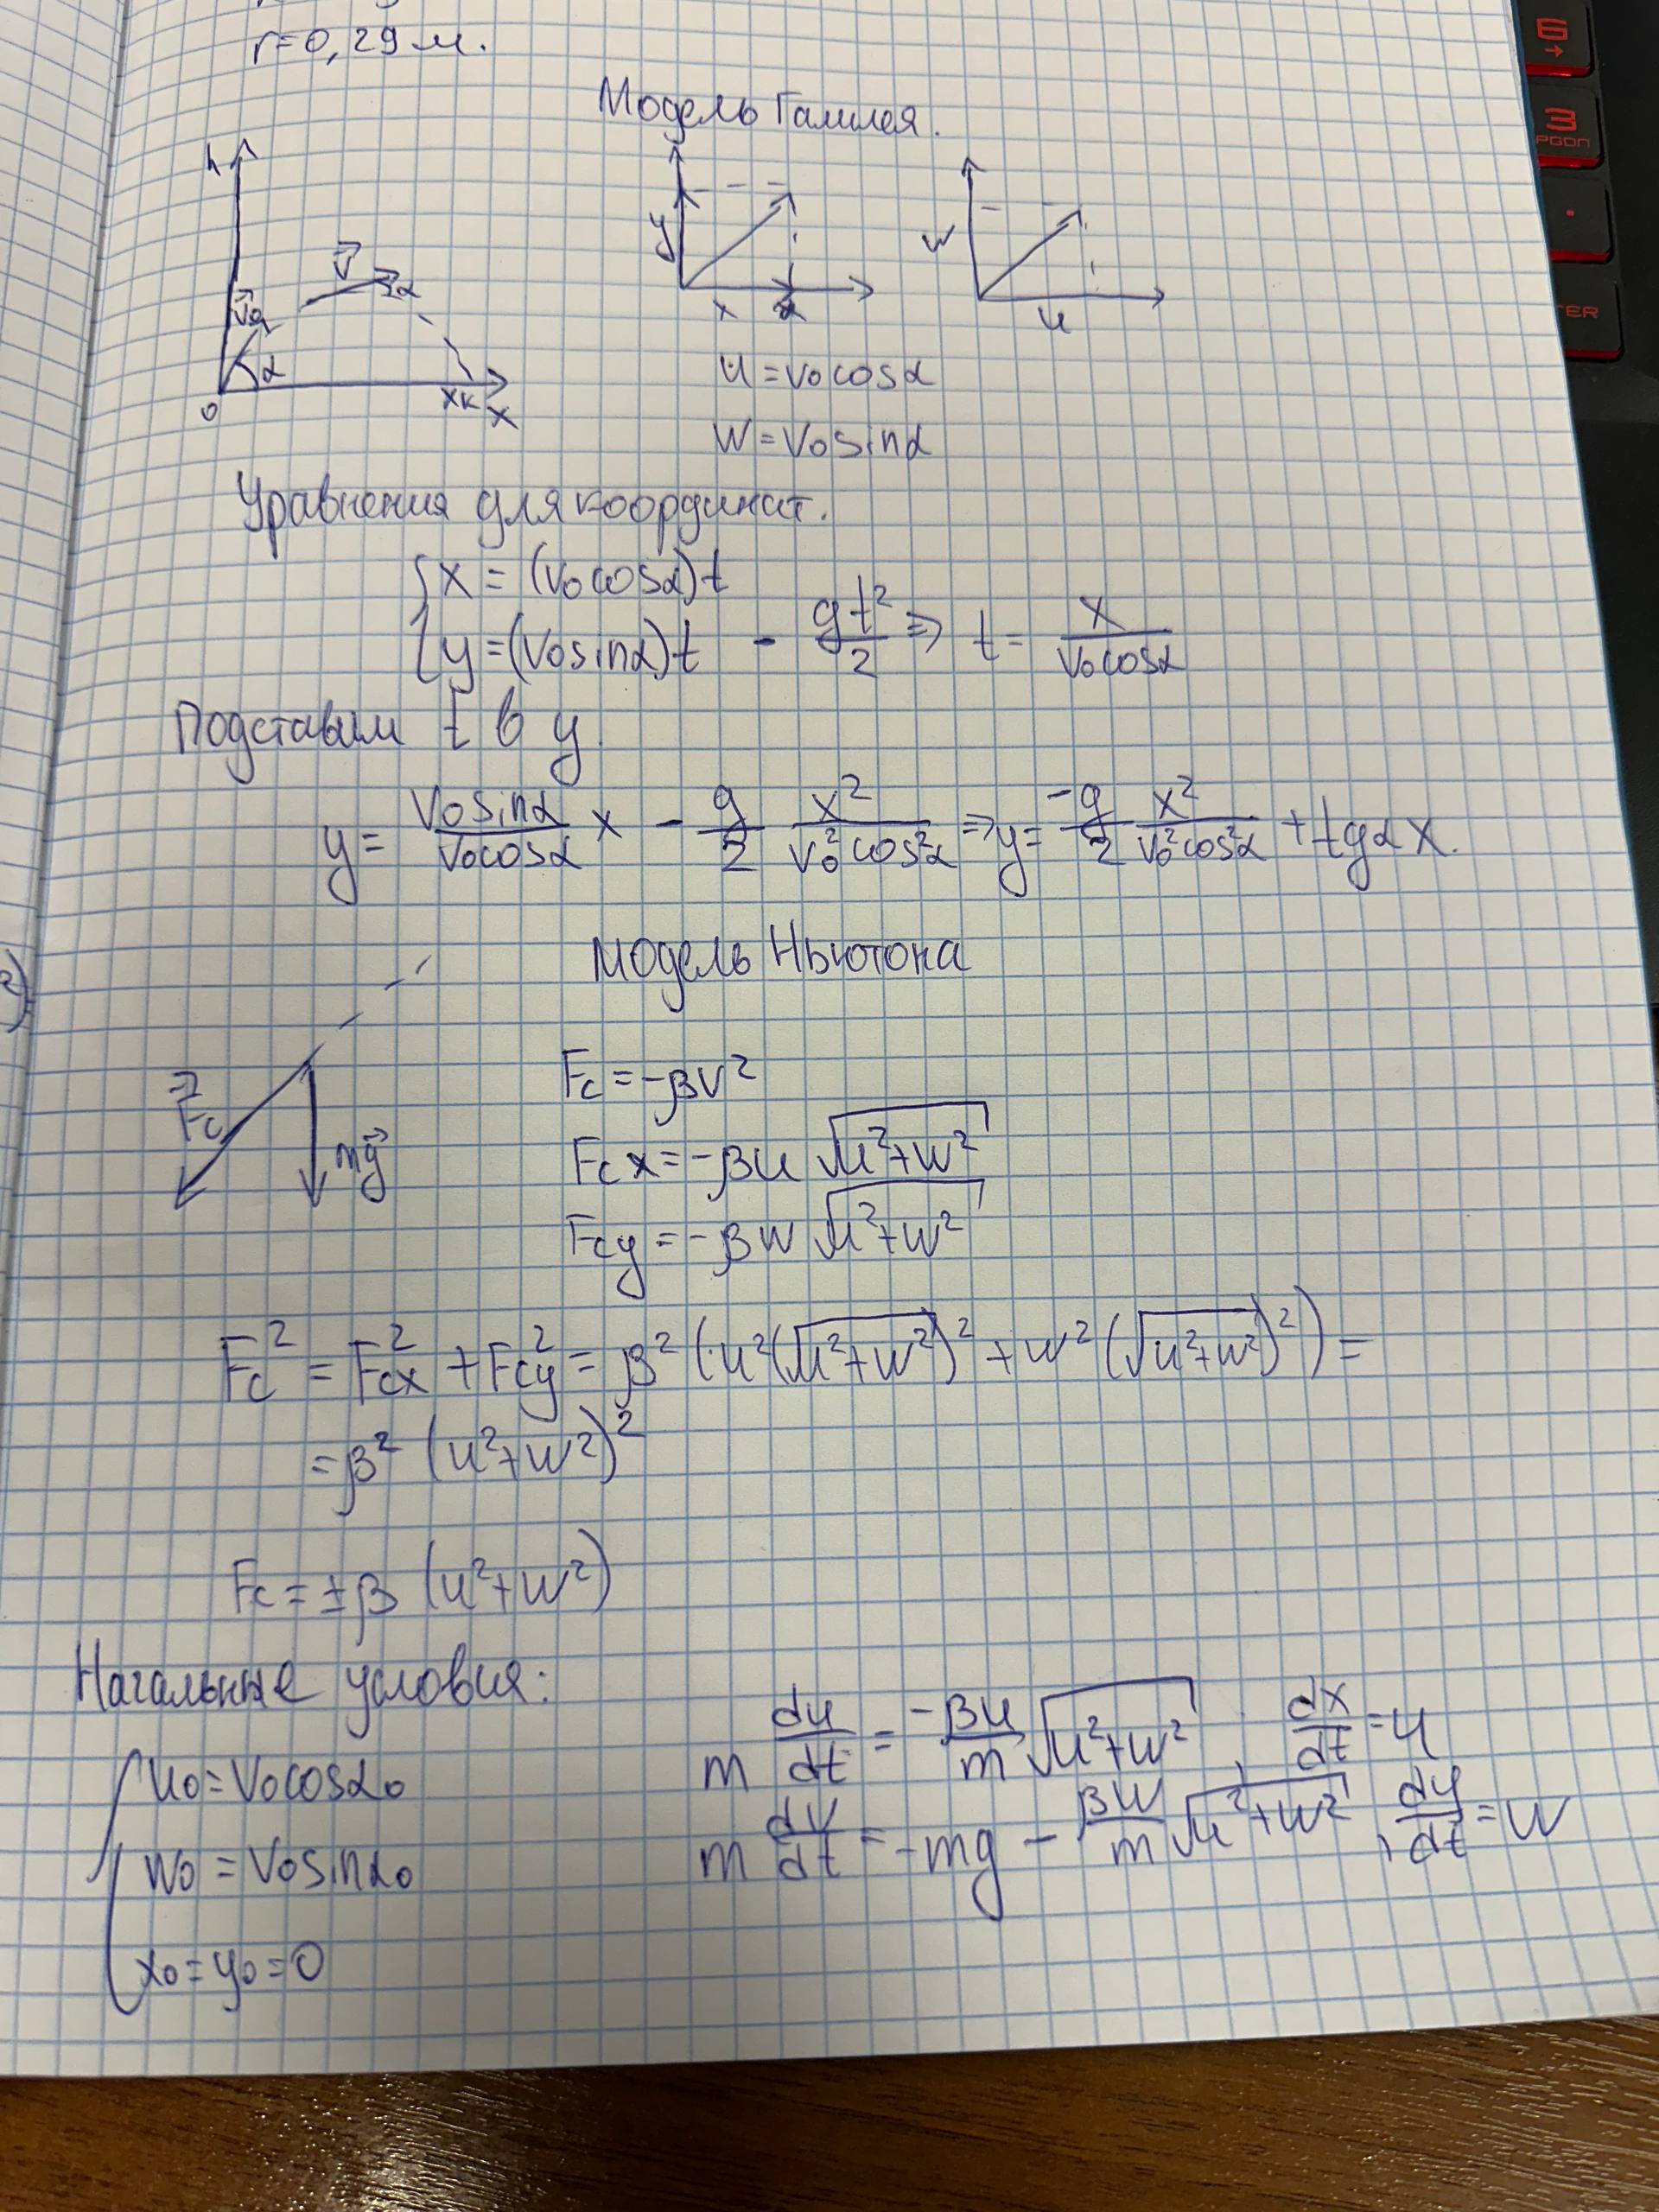
\includegraphics[width=0.85\textwidth]{model.jpg}
  \caption{Схема построения математической модели}
  \label{fig:model}
\end{figure}

\section{Разбиение на вычислительные задачи}

\subsection{Корректность вычислительной задачи}
Вычислительная задача считается корректной, если решение существует, единственно и непрерывно зависит от входных данных. В данной задаче правая часть системы ОДУ непрерывна и удовлетворяет условию Липшица по фазовым переменным в области полёта, начальные условия $x(0)=0$, $y(0)=0$, $u(0)=v_0\cos\alpha$, $w(0)=v_0\sin\alpha$ заданы однозначно. Поэтому решение задачи Коши существует и единственно при $t>0$ до момента падения на землю.

Уравнение траектории в модели Галилея при $y=0$ имеет два решения по горизонтальной координате: $x_1=0$ (точка старта в начале координат) и $x_2$~--- дальность полёта. Решение $x_1=0$ является вырожденным для задачи о дальности; физически значимо второе решение. Для модели Ньютона траектория находится численно, дальность~--- по первому пересечению $y=0$ при $t>0$.

\subsection{Решение системы ОДУ методом Рунге-Кутты}
Система обыкновенных дифференциальных уравнений решается методом Рунге-Кутты 4-го порядка. Для уравнения $\frac{dy}{dt} = f(t, y)$ на шаге $h$ по времени вычисляются четыре наклона и новое значение:
\begin{equation*}
k_1 = f(t_n, y_n),
\end{equation*}
\begin{equation*}
k_2 = f(t_n + \frac{h}{2}, y_n + \frac{h}{2}k_1),
\end{equation*}
\begin{equation*}
k_3 = f(t_n + \frac{h}{2}, y_n + \frac{h}{2}k_2),
\end{equation*}
\begin{equation*}
k_4 = f(t_n + h, y_n + h k_3),
\end{equation*}
\begin{equation*}
y_{n+1} = y_n + \frac{h}{6}(k_1 + 2k_2 + 2k_3 + k_4).
\end{equation*}
На каждом шаге по текущему состоянию $(x, y, u, w)$ вычисляются четыре вспомогательных вектора наклонов, комбинация которых даёт приближение на следующем шаге. Метод имеет четвёртый порядок точности по шагу и устойчив при разумном выборе шага интегрирования.

Линейная интерполяция на последнем шаге модели используется для уточнения точки падения: численная траектория переходит с положительной высоты на отрицательную между двумя узлами сетки. По двум последним точкам $(x_{\text{prev}}, y_{\text{prev}})$ и $(x, y)$ строится линейная интерполяция по времени, находится момент и координата пересечения с $y=0$, после чего в траекторию записывается эта точка приземления и возвращается уточнённая дальность полёта.

\section{Анализ модели}

График траекторий для варианта 29 (угол $53°$, $v_0 = 185$ м/с, железо, $r = 0{,}29$ м) представлен на рисунке~\ref{fig:trajectory}.

\begin{figure}[H]
  \centering
  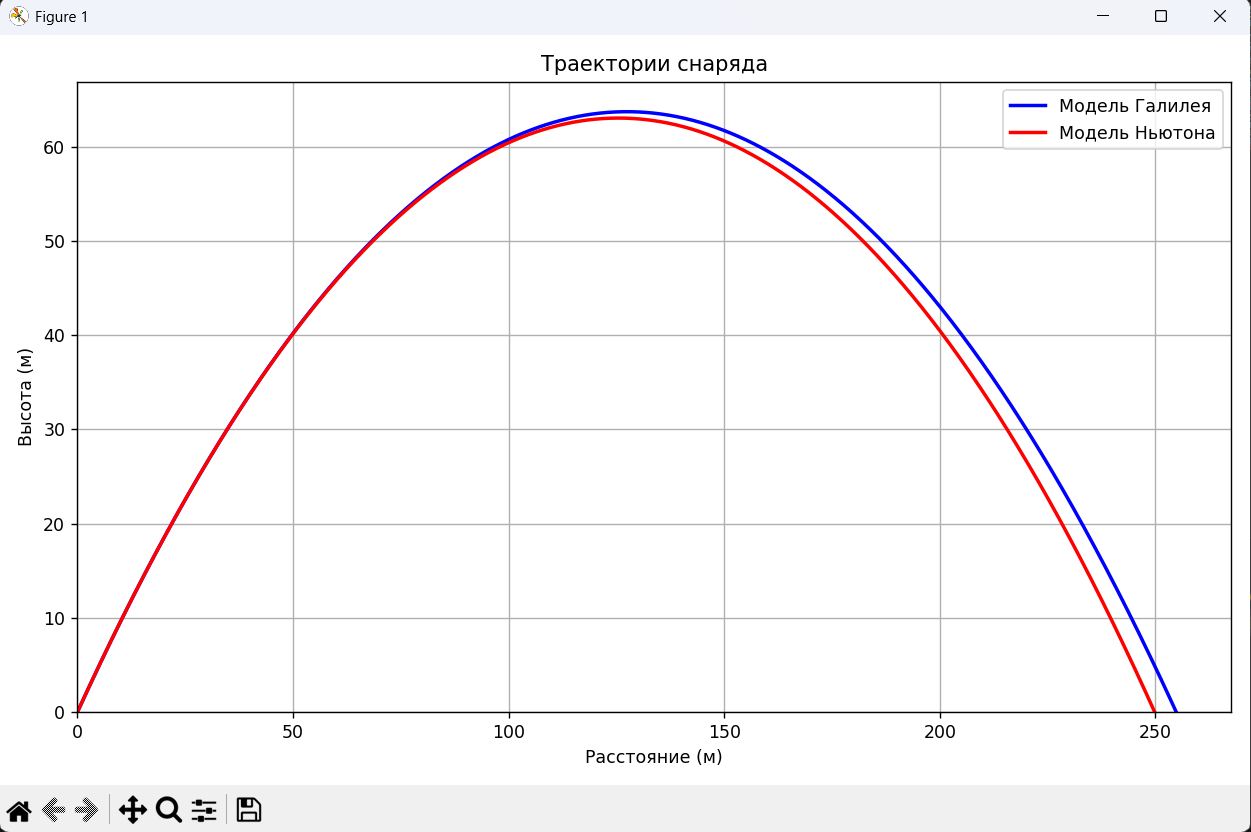
\includegraphics[width=0.75\textwidth]{screen2.png}
  \caption{Траектории полёта: модель Галилея и модель Ньютона}
  \label{fig:trajectory}
\end{figure}

\section{Вывод}

Модель Ньютона даёт меньшую дальность полёта по сравнению с моделью Галилея из-за сопротивления воздуха; траектория с сопротивлением отклоняется от параболы и раньше пересекает ось абсцисс. Учёт сопротивления воздуха необходим при расчёте траекторий реальных снарядов.

\section{Практическая реализация}

\refstepcounter{lstlisting}\label{lst:code}
\noindent\textbf{Листинг~\ref{lst:code}.} Исходный код программы.

\begin{breakablelisting}
import numpy as np
import matplotlib.pyplot as plt

def rk4_step(f, t, y, dt):
    k1 = f(t, y)
    k2 = f(t + dt/2, y + k1*dt/2)
    k3 = f(t + dt/2, y + k2*dt/2)
    k4 = f(t + dt, y + k3*dt)
    return y + dt*(k1 + 2*k2 + 2*k3 + k4)/6

def newton(v0, alpha, material_density=7000, air_density=1.225, C=0.15, dt=0.001, g=9.81):
    S = 0.03
    radius = (S/np.pi)**0.5
    m = material_density * (4/3) * np.pi * radius**3
    beta = C * air_density * S / 2.0
    u = v0 * np.cos(alpha)
    w = v0 * np.sin(alpha)
    x = 0.0
    y = 0.0
    t = 0.0
    max_t = max(4 * v0 * np.sin(alpha) / g, 30.0)
    x_prev, y_prev = x, y
    trajectory_x = [x]
    trajectory_y = [y]
    while t < max_t:
        state = np.array([x, y, u, w])
        def f(t0, s):
            ux, yy, uu, ww = s
            V = np.sqrt(uu*uu + ww*ww)
            if V < 1e-12:
                du = 0.0
                dw = -g
            else:
                du = -beta * uu * V / m
                dw = -g - beta * ww * V / m
            return np.array([uu, ww, du, dw])
        new = rk4_step(f, t, state, dt)
        x_prev, y_prev = x, y
        x, y, u, w = new
        trajectory_x.append(x)
        trajectory_y.append(y)
        t += dt
        if y < 0:
            if y == y_prev:
                return x, trajectory_x, trajectory_y
            frac = -y_prev / (y - y_prev)
            final_x = x_prev + frac*(x - x_prev)
            trajectory_x[-1] = final_x
            trajectory_y[-1] = 0.0
            return final_x, trajectory_x, trajectory_y
    return x, trajectory_x, trajectory_y

def galilei(v0, alpha, g=9.81):
    range_gal = v0*v0 * np.sin(2*alpha) / g
    t_max = 2 * v0 * np.sin(alpha) / g
    t_array = np.linspace(0, t_max, 1000)
    x_array = v0 * np.cos(alpha) * t_array
    y_array = v0 * np.sin(alpha) * t_array - 0.5 * g * t_array**2
    return range_gal, x_array.tolist(), y_array.tolist()

if __name__ == '__main__':
    alpha_deg = float(input('Угол к горизонту: '))
    v0 = float(input('Начальная скорость: '))
    alpha = np.deg2rad(alpha_deg)
    
    range_gal, x_gal, y_gal = galilei(v0, alpha)
    range_newt, x_newt, y_newt = newton(v0, alpha)
    diff = range_gal - range_newt
    
    print(f'Дальность полёта (модель Галилея): {range_gal:.6f} м')
    print(f'Дальность полёта (модель Ньютона): {range_newt:.6f} м')
    print(f'Разница: {diff:.6f} м')
    
    plt.figure(figsize=(10, 6))
    plt.plot(x_gal, y_gal, 'b-', linewidth=2, label='Модель Галилея')
    plt.plot(x_newt, y_newt, 'r-', linewidth=2, label='Модель Ньютона')
    plt.xlabel('Расстояние (м)')
    plt.ylabel('Высота (м)')
    plt.title('Траектории снаряда')
    plt.grid(True)
    plt.legend()
    plt.xlim(left=0)
    plt.ylim(bottom=0)
    plt.tight_layout()
    plt.show()
\end{breakablelisting}

\end{document}
